%    Maciej Woloszyn AGH Krakow <woloszyn@agh.edu.pl> (c) 2010
%
%    This program is free software: you can redistribute it and/or modify
%    it under the terms of the GNU General Public License as published by
%    the Free Software Foundation, either version 3 of the License, or
%    (at your option) any later version.
%
%    This program is distributed in the hope that it will be useful,
%    but WITHOUT ANY WARRANTY; without even the implied warranty of
%    MERCHANTABILITY or FITNESS FOR A PARTICULAR PURPOSE.  See the
%    GNU General Public License for more details.
%
%    You should have received a copy of the GNU General Public License
%    along with this program.  If not, see <http://www.gnu.org/licenses/>.


% run (pdf)latex on this file to produce screen version of the presentation


% include instructions shared by screen and printout versions
../_share_/shared.tex

% set page geometry (you may want to change papersize to scale fonts easily or change proportions)
\usepackage[papersize={100mm,75mm},margin=4mm]{geometry}

\setlength\parindent{0cm}
%\addtolength{\parskip}{\baselineskip}
\setlength\itemindent{0cm}
\setlength\itemsep{0cm}
\setlength\leftmargin{0cm}

% no pagenumbers, headers etc.
\pagestyle{empty}

% turn off hyphenation
\hyphenpenalty=100000

% produce new page (\newslide does nothing in the printout version)
\let\newslide=\newpage

% sans font
\renewcommand{\rmdefault}{\sfdefault}

% command for screen-only content
\newcommand{\SCR}[1]{#1}

% command for printout-only content
\newcommand{\PRN}[1]{\relax}

% title page
\newcommand{\makeslidetitle}[1]
{%
\hypersetup{pdftitle={Presentation - part #1}}
\title{Presentation\\{\normalfont part #1}}
\author{Maciej Wołoszyn\\
AGH Kraków\\
{\small \url{woloszyn@agh.edu.pl}}\\
{\small \url{http://home.agh.edu.pl/woloszyn}}}
\date{}
\setcounter{chapter}{#1}
\maketitle
\newpage
}

\sloppy

% include the content
\begin{document}
% Maciej Woloszyn AGH Krakow <woloszyn@fatcat.ftj.agh.edu.pl> (c) 2010

\makeslidetitle{99}

\section{Creating slides}
\begin{itemize}
\item 
\verb|\newslide| produces \verb|\newpage| in the file
used for presentation, while being ignored for printout PDF
\item 
\verb|\SCR{foo}|  $\leftarrow$ (\SCR{\texttt{foo}}) will be visible only in the
'screen' PDF
\item 
\verb|\PRN{foo}|  $\leftarrow$ (\PRN{\texttt{foo}}) will be visible only in the
'printout' PDF
\end{itemize}

\newslide

\section{Presenting source code}


\subsection{Including files}
\verb|\lstinputlisting{src/Hello.java}|\\
$\to$
\lstinputlisting{src/Hello.java}
\newslide
\verb|\lstinputlisting[firstline=2,lastline=3]%|\\
\verb|   {src/Hello.java}|\\
\verb|\outinclude{src/Hello.out}|\\
$\to$
\lstinputlisting[firstline=2,lastline=3]{src/Hello.java}
\outinclude{src/Hello.out}

\subsection{Inline}
$\alpha$ \code{int n=1;} for..  $\leftarrow$ \verb|$\alpha$ \code{int n=1;} for..|\\

\newslide
\subsection{lstlisting environment}
\begin{lstlisting}
class A {
  public String toString() {
    return "class A object";
  }
}
\end{lstlisting}
\begin{lstlisting}
System.out.println(new A());
\end{lstlisting}
\out{class A object}
\SCR{~\\~\\~\\~\\~\\}
is produced from:
\newslide

\begin{verbatim}
\begin{lstlisting}
class A {
  public String toString() {
    return "class A object";
  }
}
\end{lstlisting}
\begin{lstlisting}
System.out.println(new A());
\end{lstlisting}
\out{class A object}
\end{verbatim}

%%% \end{verbatim}

\newslide

\begin{lstlisting}
12345678901234567890123456789012345678901234567890
2--------1---------2---------3---------4---------5
3
4
5
6
7              rows and columns available
8               for the default settings
9
10
11
12
13
14
15
16
\end{lstlisting}

\newslide

\subsection{outlisting environment}
\begin{verbatim}
\begin{lstlisting}
some code
\end{lstlisting}
\begin{outlisting}
1st line of results
2nd line of results
\end{outlisting}
\end{verbatim}

$\to$

\begin{lstlisting}
some code
\end{lstlisting}
\begin{outlisting}
1st line of results
2nd line of results
\end{outlisting}

\newslide
\section{Other commands}


\concept{concept} $\leftarrow$ \verb|\concept{concept}|\\
\underl{underl} $\leftarrow$ \verb|\underl{underl}|\\
~\\
\stdin{interactive input} $\leftarrow$ \verb|\stdin{interactive input}|\\
~\\
\Q{how ..} $\leftarrow$ \verb|\Q{how ..}|\\
\W{note ..} $\leftarrow$ \verb|\W{note ..}|\\
~\\
\TODO{add ..} $\leftarrow$ \verb|\TODO{add ..}|\\

\newslide
\section{Outcome}
\begin{center}
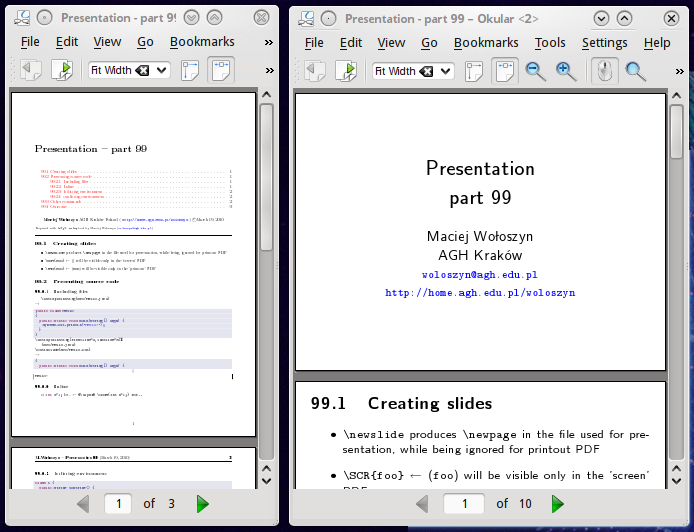
\includegraphics[width=0.8\textwidth]{fig/final}
\end{center}


\end{document}
